\documentclass{article}
% translate with >> pdflatex -shell-escape <file>

% This file is used as unit test for pgfplots, copyright by Christian Feuersaenger.
% 
% See
%   http://pgfplots.sourceforge.net/pgfplots.pdf
% for pgfplots.
%
% Any required input files (for <plot table> or <plot file> or the table package) can be downloaded
% at
% http://www.ctan.org/tex-archive/graphics/pgf/contrib/pgfplots/doc/latex/
% and
% http://www.ctan.org/tex-archive/graphics/pgf/contrib/pgfplots/doc/latex/plotdata/

\usepackage{pgfplots}
\pgfplotsset{compat=newest}

\pagestyle{empty}

\begin{document}
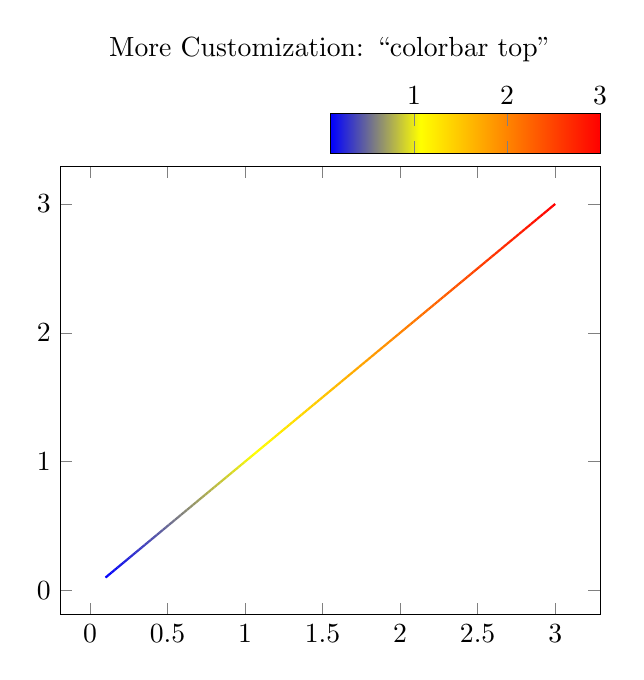
\begin{tikzpicture}
	\begin{axis}[colorbar horizontal, colorbar style={at={(1,1.03)},anchor=south east,width=0.5*\pgfkeysvalueof{/pgfplots/parent axis width},xticklabel pos=right},
	title style={yshift=1cm},
	title=More Customization: ``colorbar top'',
	]
	\addplot[mesh,thick,samples=150,domain=0.1:3] 
		{x};
	\end{axis}
\end{tikzpicture}
\end{document}
